\chapter{Analisis}
\label{chap:analisis}

\section{Deskripsi Masalah}
\label{sec:deskripsimasalah}

\hspace{0,5cm}Untuk mengolah keuangan sebuah rumah tangga tidaklah mudah. Rumah tangga memiliki beberapa anggota yang terdiri dari kepala, pengurus dan anggota(anak) rumah tangga. Tentunya pengololahan rumah tangga dilakukan oleh kepala rumah tangga atas semua transaksi keuangan yang dilakukan oleh anggota rumah tangga. Untuk melaporkan semua transaksi yang dilakukan oleh anggota rumah tangga kepada kepala rumah tangga terkadang terhalang oleh komunikasi apalagi jika kepala dan anggota rumah tangga tinggal ditempat yang berbeda.

Dari masalah tersebut, akan dibuat suatu aplikasi yang dapat membantu suatu rumah tangga dalam pengelolaan keuangan mereka. Aplikasi ini dapat digunakan oleh setiap anggota rumah tangga untuk mencatat semua transaksi yang mereka lakukan baik pengeluaran maupun pendapatan. Aplikasi ini juga dapat menampilkan laporan sesuai dengan transaksi yang telah tercatat.

Aplikasi ini sendiri terbagi menjadi dua bagian yaitu aplikasi \textit{end-user} yang digunakan langsung oleh para anggota rumah tangga dan aplikasi yang digunakan oleh admin untuk mengelolah data-data aplikasi.

Data-data yang tercatat tentunya akan disimpan kedalam sebuah basis data sehingga aplikasi ini sendiri akan berkomunikasi dengan \textit{server} yang berfungsi sebagai penyimpanan dan pengolahan data yang dibangun diatas \textit{framework} Hadoop. Untuk komunkasi aplikasi dan \textit{server} akan menggunakan HTTP dimana aplikasi akan mengakses \textit{webservice} yang telah disediakan oleh \textit{server}.

\section{\textit{Mobile Cloud Computing Model} untuk Pembukuan Rumah Tangga}

Pada permodelan dipenelitian ini menggunakan \textit{Mobile Cloud Computing Model} dimana aplikasi akan berkomunikasi dengan \textit{server} melalui \text{webservice} diatas HTTP. \textit{Webservice} akan gerbang bagi aplikasi untuk memanipulasi data. Untuk bagian \textit{back-end}, \textit{webservice} akan ditulis di atas PHP dan menggunakan Trafodion untuk memanipulasi data diatas Hadoop. Gambaran model dapat dilihat pada Gambar~\ref{fig:prt_architecture}

\begin{figure}[h]
\centering
\resizebox{\textwidth}{!}{
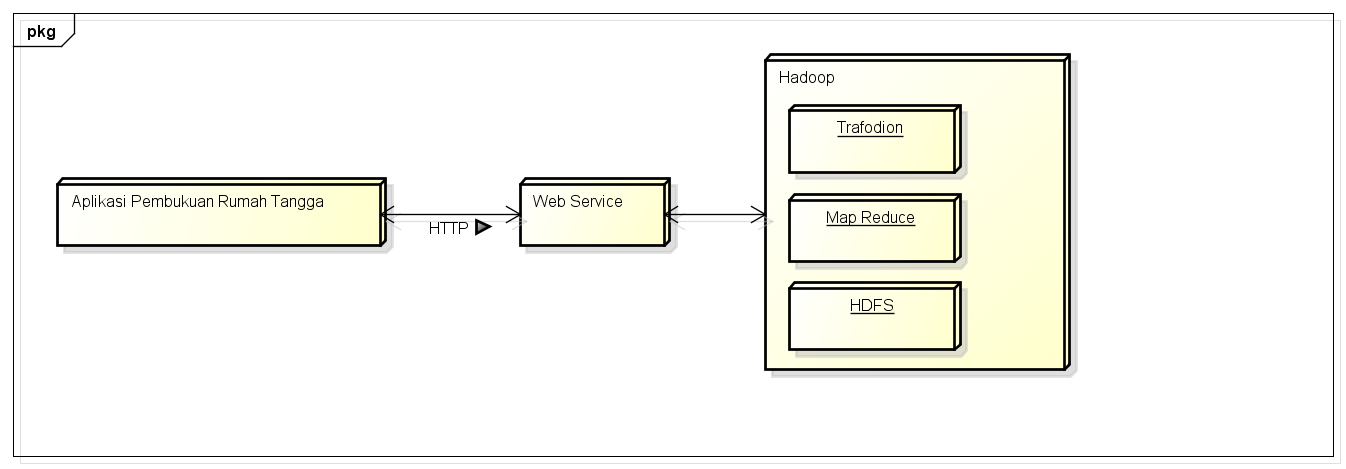
\includegraphics{Gambar/prt-architecture}
}
\caption[Permodelan Pembukuan Rumah Tangga]{Permodelan Pembukuan Rumah Tangga} 
\label{fig:prt_architecture}
\end{figure}

\section{Analisis Kebutuhan Perangkat Lunak}

\hspace{0,5cm}Pada sub-bab ini akan dibahas mengenai analisis terhadap perangkat lunak yang akan dikembangkan.

\subsection{Analisis Aplikasi \textit{Mobile Device}}

Pada aplikasi \textit{mobile device} akan ditujukan kepada pengguna rumah tangga untuk mengelolah transaksi yang mereka lakukan. Aplikasi ini memiliki beberapa fitur utama dan tiga peran.

\hspace{0,5cm}Peran yang ada pada aplikasi ini yakni:
\begin{enumerate}
	\item Kepala rumah tangga
	\item	Pengurus rumah tangga
	\item Anggota rumah tangga
\end{enumerate}

Fitur-fitur yang ada, yakni:
\begin{enumerate}
	\item Pendaftaran diri, pendaftaran dilakukan untuk mendapatkan hak akses kedalam sistem aplikasi dan pendaftaran mendapat peran sebagai kepala rumah tangga
	\item Pengisian profil rumah tangga, pengisian profil dilakukan oleh kepala rumah tangga setelah mendaftarkan diri dan disetujui oleh admin
	\item	Mendaftarkan pengurus dan anggota rumah tangga, kepala rumah tangga dapat menambahkan dan mengurungai pengurus dan anggota rumah tangga yang berelasi terhadapnya
	\item Mencatat transaksi, semua peran mendapat hak akses untuk fitur ini dimana fitur ini untuk mencatat transaksi keuangan masing-masing.
	\item Alokasi keuangan, fitur ini berupa transfer dana antar anggota rumah tangga, baik dari kepala ke anggota dan sebaliknya, fitur ini hanya dimiliki oleh kepala dan pengurus rumah tangga.
	\item Menambah kategori transaksi, fitur ini hanya dimiliki oleh kepala rumah tangga yang bertujuan untuk menambah kategori transaksi.
	\item Melihat laporan keuangan, fitur ini hanya dapat diakses oleh kepala dan penguru rumah tangga.
	\item Melihat transaksi, fitur ini dapat diakses oleh semua peran rumah tangga.
\end{enumerate}

Penulis akan mengembangkan aplikasi \textit{mobile device} menggunakan Phonegap yang ditulis diatas \textit{webview} tetapi aplikasi ini tidak akan berjalan diatas \textit{web browser} karena Phonegap yang akan meng-\textit{compile} aplikasi ini sehingga akan menjadi suatu aplikasi Android.Untuk tampilan dasar pada aplikasi, penulis menggunakan \textit{framework} Onsen-UI yang dibangun diatas AngularJS. Penulis memilih \textit{framework} ini karena merupakan \textit{single page web} yang cocok untuk membuat aplikasi yang hendak dibangun penulis. Selain menggunakan AngularJS, penulis juga mengguna Jquery untuk memanipulasi data pada aplikasi.


\subsection{Analisis Aplikasi \textit{Website}}

\hspace{0,5cm}Aplikasi \textit{website} ini dibuat hanya untuk admin sehingga dapat mengatur data-data yang ada pada aplikasi.

Fitur-fitur yang ada yakni:
\begin{enumerate}
	\item Pengolahan anggota
				Admin dapat menyetujui atau menolak pendaftaran dari pengguna
	\item	Pengolahan kategori transaksi
				Admin dapat mengurangi atau menambah kategori transaksi
	\item Pelaporan
				Admin dapat membuat laporan secara keseluruhan
\end{enumerate}

Penulis akan mengembangkan aplikasi \textit{website} menggunakan \textit{framework} CakePHP yang ditulis diatas PHP. CakePHP mengikuti disain MVC yang memudahkan untuk membuat suatu aplikasi \textit{website}.

Pada aplikasi ini, terdapat beberapa model berupa:
\begin{itemize}
	\item Anggota yang merepresentasikan anggota pengguna aplikasi \textit{mobile device.}
	\item Kategori yang merepresentasikan kategori-kategori transaksi yang ada.
	\item Rumah Tangga yang merepresentasikan sebuah rumah tangga
	\item Transaksi yang merepresentasikan transaksi yang dilakukan oleh anggota.
	\item Account yang merepresentasikan akun pengguna aplikasi \textit{website}.
	\item Module yang merepresentasikan menu yang ada pada aplikasi \textit{website}.
	\item ModuleContent yang merepresentasikan sub-sub menu yang ada pada aplikasi \textit{website}.
	\item User yang merepresentasikan data login untuk akun pengguna aplikasi \textit{website}.
	\item UserGroup yang merepresentasikan grup akun.
	\item Role yang merepresentasikan hak akses setiap UserGroup.
\end{itemize}

\subsection{Analisis \textit{Webservice}}

\hspace{0,5cm}Aplikasi \textit{mobile device} membutuhkan fungsi-fungsi untuk memanipulasi data. Fungsi-fungsi ini dapat dibangun pada aplikasi \textit{website} dan biasanya disebut dengan \textit{webservice}. Penulis akan membuat webservice yang berfungsi menyediakan layanan untuk aplikasi \textit{mobile device}. Penulis akan membangun webservice diatas PHP, mengikuti disain REST dan menggunakan JSON sebagai respon format data.

Adapun beberapa layanan yang akan dibuat berupa:
\begin{itemize}
	\item Mencatat transaksi.
	\item Menambah dan mengurangi kategori transaksi.
	\item Menyiapkan data laporan.
	\item Melihat anggota rumah tangga.
\end{itemize}

\subsection{\textit{Use Case}}

\hspace{0,5cm}Proses yang akan dilalui dalam bisnis ini berupa:
\begin{enumerate}
	\item Administrator menentukan katagori transaksi yang dapat dipakai oleh semua rumah tangga.
	\item Kepala rumah tangga mendaftarkan diri ke sistem.
	\item Administrator memverifikasi dan menyetujui pendaftaran Kepala rumah tangga.
	\item Kepala rumah tangga yang sudah disetujui pendaftarannya, melengkapi data profil rumah tangganya.
	\item Kepala rumah tangga mendaftarkan pengurus dan anggota rumah tangganya.
	\item Kepala rumah tangga dapat menambahkan atau mengurangi katagori transaksi keuangan yang dapat digunakan dalam rumah tangganya.  
	\item Kepala rumah tangga dapat mengalokasikan katagori transaksi keuangan di dalam rumah tangganya kepada pengurus dan anggota rumah tangga.
	\item Kepala atau pengurus rumah tangga dapat mentransfer uang dari akun induk ke akun anggota rumah tangga.
	\item Kepala atau pengurus rumah tangga dapat memonitor semua transaksi rumah tangganya melalui laporan rumah tangganya.
	\item Semua anggota rumah tangga (termasuk Kepala dan Pengurus) dapat melakukan transaksi keuangan sesuai dengan katagori transaksi keuangan yang telah dialokasikan kepadanya.
\end{enumerate}

\hspace{0,5cm}Diagram \textit{use case} oleh pengguna aplikasi dapat dilihat pada Gambar~\ref{fig:diagram_use_case_mobile}

\begin{figure}[h]
\centering
\resizebox{\textwidth}{!}{
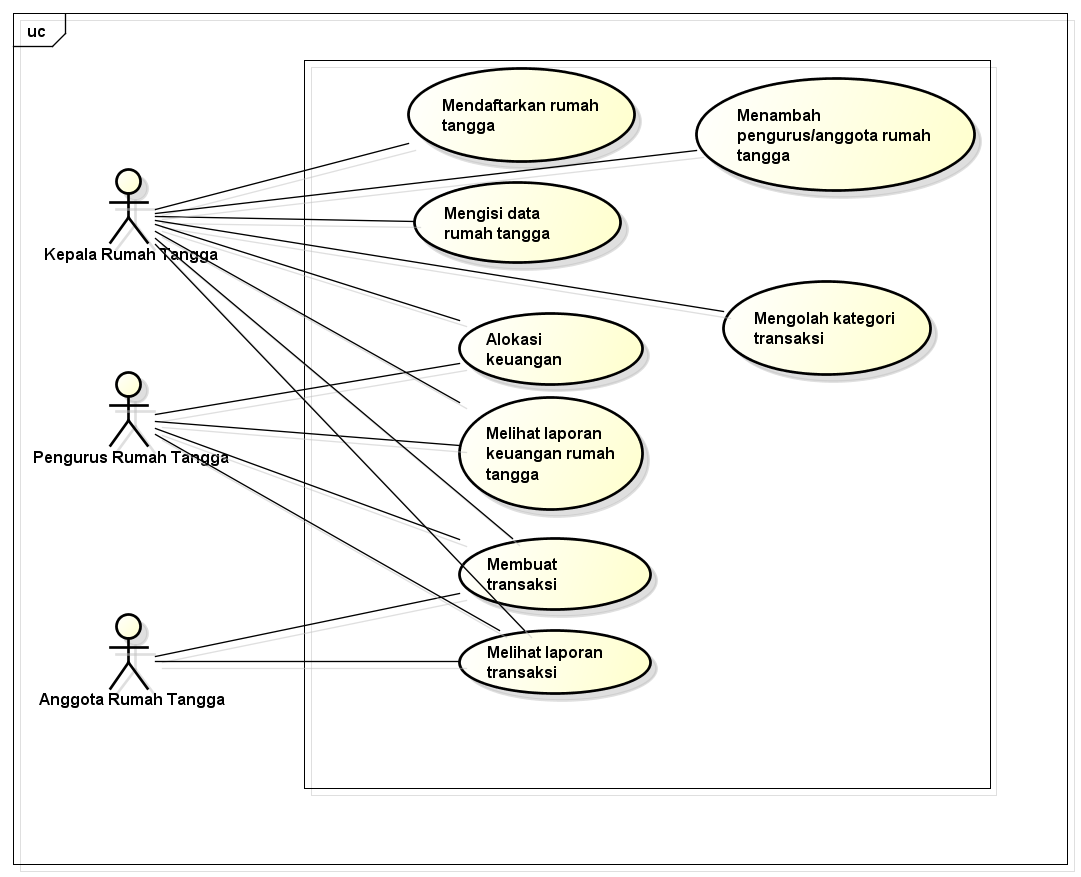
\includegraphics[scale=0.02]{Gambar/use-case-mobile}
}
\caption[Diagram \textit{Use Case Mobile Device}]{Diagram \textit{Use Case Mobile Device}} 
\label{fig:diagram_use_case_mobile}
\end{figure}

Diagram \textit{use case website} yang digunakan admin dapat dilihat pada Gambar~\ref{fig:diagram_use_case_website}

\begin{figure}[h]
\centering
\resizebox{\textwidth}{!}{
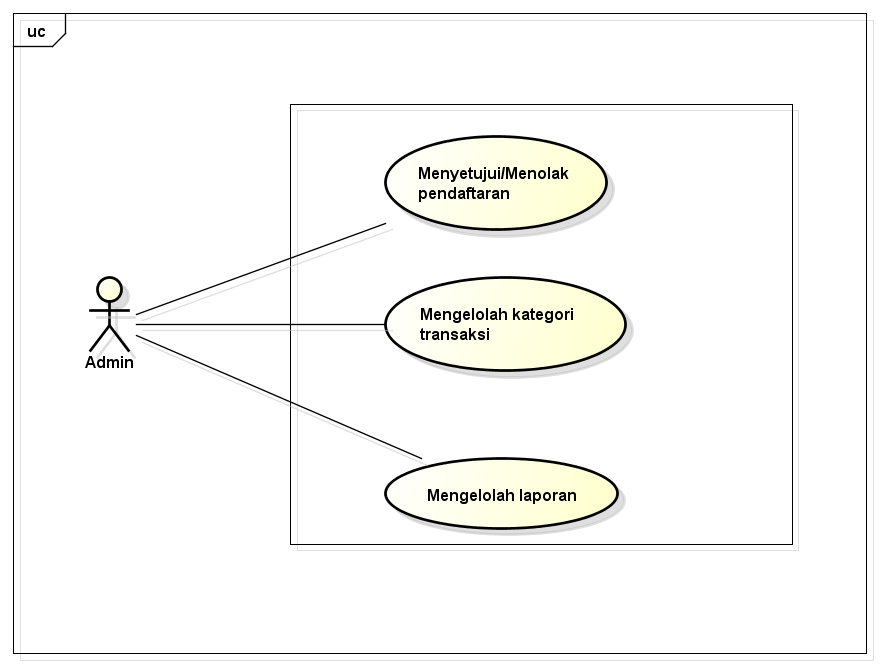
\includegraphics[scale=0.02]{Gambar/use-case-web}
}
\caption[Diagram \textit{Use Case Mobile Website}]{Diagram \textit{Use Case Mobile Website}} 
\label{fig:diagram_use_case_website}
\end{figure}